% BioDecisionBench — working draft (venue unbound; article+geometry paradigm
% shared with the previous Laya-Bio manuscript, so it compiles without any
% venue style file. Swap the preamble when the venue is fixed.)
\documentclass[10pt]{article}
\usepackage[letterpaper,margin=0.85in]{geometry}
\usepackage[T1]{fontenc}
\usepackage[utf8]{inputenc}
\usepackage{lmodern}
\usepackage{amsmath,amssymb,booktabs,graphicx,microtype}
\usepackage[round,authoryear]{natbib}
\usepackage{xurl}
\usepackage[hidelinks]{hyperref}
\usepackage[capitalize,noabbrev]{cleveref}
\usepackage{caption}
\captionsetup{font=small,labelfont=bf}
\usepackage{xcolor}
\usepackage{multirow}
\setlength{\parskip}{2pt}
\setlength{\textfloatsep}{12pt plus 2pt minus 2pt}
\setlength{\intextsep}{10pt plus 2pt minus 2pt}
\setlength{\tabcolsep}{5pt}
\graphicspath{{figures/}}
% Shared notation for BioDecisionBench
\newcommand{\R}{\mathbb{R}}
\newcommand{\E}{\mathbb{E}}
\DeclareMathOperator*{\argmax}{arg\,max}
\newcommand{\task}{t}
\newcommand{\famof}[1]{\mathcal{F}(#1)}
\newcommand{\prim}{p}
\newcommand{\metric}{m}
% architecture labels used inline: \arch{1} -> #1
\newcommand{\arch}[1]{\mbox{\rm\##1}}


\title{BioDecisionBench: A Leak-Proof Typed-Decision Benchmark\\for Biological Sequences, and a Seed-Averaged\\Comparison of Decision Architectures}
\author{Anonymous Authors\\(working draft — venue unbound)}
\date{October 2026}

\begin{document}
\maketitle

\begin{abstract}
Can one model answer ``is this promoter active?'' (a yes/no judgement), ``which fold does
this protein adopt?'' (a choice among labels), and ``how fit is this mutant?'' (an ordinal
score) through a single decision interface? Typed-decision interfaces --- which encode the
question and the candidate answers as text and let one \emph{shared scorer} rank candidates,
with no per-task output heads --- are being adopted for exactly this setting, but have never
been compared against conventional task heads under matched compute. We release
\textbf{BioDecisionBench}: 290 biological sequence decision tasks spanning DNA, protein and
RNA, unified under four typed decision primitives --- Noul (yes/no judgement), Choice
(mutually exclusive labels), Score (ordinal value), and multi-Noul (multi-label) --- with a
leak-proof admission protocol that keeps legacy blind-test sets verbatim, quarantines
1{,}984 conflicting-label groups instead of majority-voting them, and verifies zero
within-task train/test sequence overlap. On this benchmark we run, to our knowledge, the
first seed-averaged three-way comparison of decision architectures: a shared typed-decision
scorer, per-task heads on the same encoder, and a frozen small language model scored by
full-candidate likelihood. Averaged over three seeds, per-task heads match or beat the
shared scorer --- Noul AUROC $0.629\pm0.050$ vs.\ $0.478\pm0.051$ (disjoint SEMs), Choice and
Score at parity --- while the shared scorer is markedly less stable (run-std 0.087 vs
0.030). The shared scorer's claimed advantages survive only qualitatively: its zero-shot
transfer is at the level of the untrained base, its cross-family transfer is weak
($+0.036\pm0.034$, classification only), and a fresh task head catches its zero-shot
performance with ${\approx}32$ labels. Single-run differences of $\pm0.05$--$0.1$ reverse
architectural conclusions in this regime; we document a complete case in which a
single-run verdict is reversed by seed averaging, and propose $\ge3$-seed averaging with
run-std reporting as the minimum bar for such comparisons.
\end{abstract}

\section{Introduction}
\label{sec:intro}

A single biological sequence model should ideally answer qualitatively different questions
through one interface, and the interface can be as simple as text: present the sequence
\texttt{GTATTCTCCCCTAACAAGAC...} with the question \emph{``Is this DNA sequence a
promoter?''} and the candidates \{yes, no\}, and a model returns $P(\text{yes})$; swap only
the question and candidate set --- \{All Alpha, All Beta, Alpha and Beta, ...\} for fold
class, five value-anchored ordinal levels for mutation fitness, per-label yes/no for
subcellular localization --- and the same model, with no task-specific output heads and no
free-text generation, answers all of them. \emph{Typed-decision} interfaces implement
exactly this design. They are being adopted in
practice, by commercial systems \citep{almeida2026jev} and by open reimplementations
\citep{gliclass2025,nanojev2026,semif2025}, on the promise of one small model, dynamic
candidate sets, and zero-adaptation-cost new tasks. Yet two basic questions have never been
answered under controlled conditions. \textbf{Q1:} does a shared typed-decision scorer match
or beat conventional per-task output heads at matched compute? \textbf{Q2:} does the
``dynamic candidates / zero adaptation'' selling point translate into a measurable
performance or cost advantage?

Answering these questions runs into three obstacles. First, biological sequence evaluation
is fragmented: GUE \citep{zhou2024dnabert}, Genomic Benchmarks
\citep{gresova2022genomic}, TAPE \citep{rao2019tape}, ProteinGym \citep{notin2023proteingym}
and friends each define their own task formats, splits and metrics, so decision architectures
cannot be compared in one protocol. Second, leakage auditing is largely absent: several
upstream ``train'' pools on public hubs \emph{contain the blind-test members of prior
studies}, so a random re-split silently fabricates a new test set. Third --- the
methodological spine of this paper --- \emph{evaluation variance in this regime has never
been quantified}. In our small-budget multi-task setting, two runs of the same configuration
and seed differ by $\pm0.05$--$0.1$ on task-macro metrics, enough to reverse the winner of
an architecture comparison (\cref{sec:mainresults}). Any single-run architectural conclusion
is therefore unreliable, including our own early one.

\paragraph{Approach.}
We build a benchmark first and a measurement protocol second, then compare architectures.
BioDecisionBench converts ten source families (290 tasks; DNA, protein, RNA, and double
sequences) into one typed-decision record format with a leak-proof admission protocol
(\cref{sec:benchmark}). On a 37-task matched slice we train the two comparable arms --- a
shared typed-decision scorer (\arch{1}) and per-task heads on the same encoder (\arch{2})
--- with family-balanced interleaving, stabilized optimization, per-family dev early
stopping, and three seeds; the frozen Qwen3-0.6B full-candidate likelihood (\arch{3}) serves
as an off-the-shelf reference (\cref{sec:framework}). \Cref{sec:results} reports the
seed-averaged comparison and three operational tests of \arch{1}'s claimed value, plus
training-dynamics and mechanism ablations.

\paragraph{Contributions.}
\begin{itemize}
\item \textbf{BioDecisionBench} (\cref{sec:benchmark}): a 290-task, three-modality,
four-primitive biological decision benchmark with a leak-proof admission protocol --- exact
cross-split sequence isolation, conflict-group quarantine (1{,}984 groups, not
majority-voted), verbatim preservation of legacy blind tests, and label mappings validated
on full pool$\cap$test overlaps. Post-isolation within-task leakage is zero.
\item \textbf{A seed-averaged evaluation protocol with a documented failure of single runs}
(\cref{sec:seedavg,sec:mainresults}): same-configuration reruns differ by up to
$7\times$ on score Spearman (0.107 vs 0.015) and reverse the comparison outcome; we make
$\ge3$ seeds, per-task seed means, SEM + run-std reporting, and dev early stopping the
minimum bar for this class of comparison.
\item \textbf{The first matched-compute three-way comparison of decision architectures on
biology} (\cref{sec:mainresults,sec:value}): per-task heads $\ge$ shared scorer (Noul
significantly better, Choice/Score at parity, and more stable across seeds); both trained
arms beat the frozen candidate-likelihood baseline. The shared scorer's advantage is
\emph{qualitative} --- it can serve arbitrary new tasks with zero adaptation, but its
zero-shot quality equals the untrained base, cross-family transfer is weak and
classification-only, and ${\approx}32$ labels let a fresh head catch its zero-shot level.
\item \textbf{Training-dynamics and mechanism diagnostics} (\cref{sec:dynamics,sec:ablations}):
naive budget scaling destabilizes joint training below the untrained baseline; stabilization
recovers but confirms a plateau; per-family checkpoint selection is a zero-inference-cost
improvement (family-optimal steps span $26\times$); two reusable controlled ablations
(noul candidate phrasing across three stable checkpoints; contrastive decoding for frozen
VLM candidate likelihood).
\end{itemize}

\paragraph{Results preview.}
Seed-averaged, per-task heads reach Noul AUROC 0.629 against the shared scorer's 0.478
(SEMs disjoint) --- while a single earlier run had suggested the opposite ordering. The
shared scorer's zero-shot interface, its headline feature, is caught by a fresh 32-label
linear head on 7 of 11 held-out tasks.

\Cref{fig:hero} summarizes the benchmark and the headline comparison.

\begin{figure*}[t]
\centering
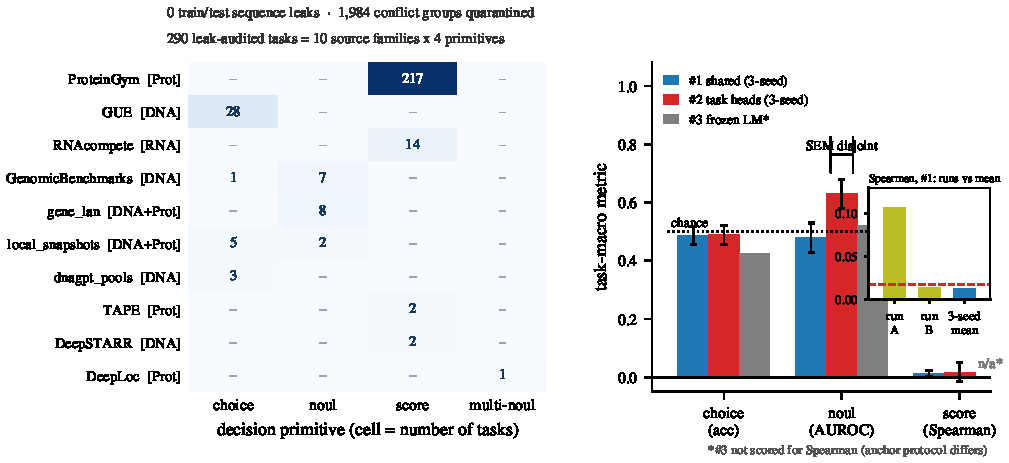
\includegraphics[width=0.90\textwidth]{fig1_hero.pdf}
\caption{\textbf{BioDecisionBench and its headline comparison.}
\emph{Left:} 290 leak-audited tasks over 10 source families and 4 decision
primitives; the admission protocol leaves zero within-task train/test sequence
overlap (1{,}984 conflicting-label groups quarantined rather than majority-voted).
\emph{Right:} seed-averaged (3 seeds), matched-compute comparison per primitive
(mean$\pm$SEM over tasks). Per-task heads (\#2) beat the shared typed-decision
scorer (\#1) on noul (disjoint SEMs) and tie on choice/score; both trained arms
exceed the frozen candidate-likelihood baseline (\#3, not compute-matched).
\emph{Inset:} the methodological warning --- two single runs of the same
configuration give score Spearman 0.107 vs 0.015 for \#1; the 3-seed mean is 0.013.}
\label{fig:hero}
\end{figure*}

\section{Related Work}
\label{sec:related}

\paragraph{Biological sequence benchmarks and foundation models.}
DNA benchmarks cover histone marks, promoters, splice sites and regulatory annotations
(GUE/DNABERT-2, 28 tasks \citep{zhou2024dnabert}; Genomic Benchmarks \citep{gresova2022genomic};
DeepSEA \citep{zhou2015deepsea}; DeepSTARR \citep{dealmeida2022deepstarr}); protein
benchmarks cover fluorescence, stability, homology and mutation-fitness assays
(TAPE \citep{rao2019tape}; ProteinGym's 217 DMS assays \citep{notin2023proteingym};
FLIP \citep{dallago2021flip}); localization and function benchmarks
are multi-label (DeepLoc 2.0 \citep{thumuluri2022deeploc}; DeepGOZero
\citep{kulmanov2022deepgozero}); RNA benchmarks cover RBP binding preference
(RNAcompete \citep{ray2013rnacompete}). Foundation models --- ESM-style protein LMs
\citep{lin2023esm2}, protein language tooling \citep{xu2023protst,xu2023biotranslator}, and
multimodal DNA agents \citep{almeida2025chatnt} --- are trained and ranked per family. These
resources are family-siloed: incompatible record formats, split protocols and metric
conventions make cross-family, cross-interface measurement impossible, and most are
single-sequence, single-task-type. BioDecisionBench is not another leaderboard substrate: it
converts these sources into one typed-decision record format with leakage auditing as a
first-class citizen (\cref{sec:admission}) and serves as the evaluation base for the
architecture comparison.

\paragraph{Typed and candidate-scoring decision interfaces.}
The Jev line of systems \citep{almeida2026jev} exposes structured Noul/Choice/Score
probabilistic judgements behind a service interface (weights not public). Open variants
include GLiClass, a ModernBERT uni-encoder with dynamic label sets
\citep{gliclass2025}; NanoJev, a small shared-scorer reimplementation
\citep{nanojev2026}; and SemIf, which reads option logits from a frozen LLM
\citep{semif2025}. Constrained decoding is the generative counterpart
\citep{scholak2021picard}. Each of these validates the interface's feasibility; none
compares \emph{shared scorer vs.\ per-task heads} under matched compute, same data, and
multiple seeds. We report the honest, counter-intuitive outcome of exactly that comparison.

\paragraph{Evaluation methodology and variance.}
Repeated runs and variance reporting are standard advice in ML evaluation
\citep{bouthillier2021variance,miller2024errorbars}; LLM-evaluation work documents
sensitivity to phrasing, prompt format and option order \citep{miller2024errorbars}. In
biology, prior work measured candidate-order sensitivity in the same decision setting:
reordering candidates changes ${\approx}9\%$ of predictions \citep{wang2026biopaws}. This paper adds a concrete \emph{conclusion-reversal}
case for architecture comparison: two runs of one configuration give score Spearman 0.107
vs 0.015 for the shared scorer, flipping the winner; three-seed averaging overturns the
single-run ``shared $\ge$ heads'' verdict (\cref{sec:mainresults}). To our knowledge this is
the first fully documented instance of run variance reversing a decision-architecture
conclusion, and we operationalize the remedy: $\ge3$ seeds, per-task seed means, SEM and
run-std reported separately, and dev early stopping with $\ge256$ dev samples.

\paragraph{Probing and adaptation cost.}
Linear probing and few-shot head fitting are standard tools for characterizing
representations. We operationalize the ``zero-adaptation interface'' claim as a
\emph{catch-up cost}: freeze the encoder, fit a new head for a held-out task with
$N\in\{32,128,512\}$ labels, and report the smallest $N$ at which the head reaches the
shared scorer's zero-shot level (\cref{sec:value}). This turns ``interface flexibility''
from a qualitative claim into a comparable number.

\section{BioDecisionBench: Design and Construction}
\label{sec:benchmark}

\subsection{Unified interface and record format}
\label{sec:schema}

Every example is one JSON line carrying
\texttt{task\_id}, \texttt{primitive}, \texttt{modality}, \texttt{sequences}
(each \texttt{\{role, modality, sequence\}}), \texttt{question}, \texttt{split},
\texttt{group}, and \texttt{provenance}, plus interface fields determined by the decision primitive
$\prim\in\{\text{noul},\text{choice},\text{score},\text{multi\_noul}\}$
(\cref{tab:primitives}). Sequences keep role boundaries for double-sequence tasks
(\texttt{query\_1}/\texttt{query\_2}: DNA+protein, DNA+DNA, protein+protein) rather than
being concatenated. \texttt{provenance} records source repository, revision/commit and
license; download receipts include per-file SHA-256.

\begin{table}[t]
\centering
\caption{The four decision primitives, their extra fields, supervision and metrics.}
\label{tab:primitives}
\small
\footnotesize
\begin{tabular}{p{0.10\textwidth}p{0.40\textwidth}p{0.36\textwidth}}
\toprule
Primitive & Extra fields & Supervision / evaluation \\
\midrule
choice & candidates (mutually exclusive labels), answer
       & CE; accuracy, macro-F1, NLL, candidate-validity rate \\
noul & candidates = \{no, yes\}, answer
     & binary CE; AUROC, MCC, accuracy, calibration \\
score & score\_levels (5), anchors (5 values from 4 interior train quantile
        cuts), gold\_value, gold\_level
      & soft-target CE + expected-value MSE; Spearman (primary), train-std-normalized
        RMSE \\
multi\_noul & candidates (all labels), per-label 0/1 vector, answer = positive set
            & masked binary; micro/macro-F1, per-label calibration \\
\bottomrule
\end{tabular}
\end{table}

\subsection{Sources, scale, and modalities}
\label{sec:scale}

\Cref{tab:benchmark} lists the composition. ProteinGym contributes 217 mutation-fitness
assays using the official contiguous-5 per-mutant folds (fold 0 = test, fold 1 = dev,
folds 2--4 = train; multi-mutant rows excluded); GUE 28 DNA choice tasks; RNAcompete 14
RNA score tasks (14-RBP subset, probes subsampled to 25k with a fixed seed); Genomic
Benchmarks 8; gene\_lan\_transfer 8 double-sequence noul tasks with endpoint
union-find component grouping; dnagpt DNA pools 3 (+1 promoter); TAPE 2; DeepSTARR 2
(dual outputs split into two tasks); DeepLoc 2.0 as one multi-noul task; and 7 local
snapshots from earlier public releases \citep{wang2024llamagene,wang2026biopaws}. Interface
distribution: choice 37 / noul 17 / score 235 / multi\_noul 1; modality: DNA 42 / protein
226 / RNA 14 / double-sequence 8; rows: 3{,}119{,}067 train / 440{,}305 dev /
581{,}242 test.

\emph{Counting convention.} The 290 figure counts evaluation units, not question types:
ProteinGym's 217 assays share one question type. We report both numbers wherever the
benchmark scale is quoted and never claim ``290 independent questions''.

% Table 1: benchmark composition (generated by gen_tables.py)
\begin{table}[t]
\centering
\caption{BioDecisionBench composition. Rows are the 10 source families (canonical
task-id prefix map used by the training scheduler; \texttt{lg\_}/\texttt{protein\_homology} share the
\texttt{local\_snapshots} family). Task counts are per evaluation unit; ProteinGym's 217 assays
share one question type. Admission: 0 train/test sequence leaks after isolation;
1{,}984 conflicting-label groups quarantined (not majority-voted);
925{,}985 cross-task duplicate sequences kept isolated per task.}
\label{tab:benchmark}
\small
\begin{tabular}{lrrrrrrrrr}
\toprule
Family & Mod. & choice & noul & score & multi & Tasks & Train & Dev & Test
\\ \midrule
ProteinGym & P & -- & -- & 217 & -- & 217 & 415,201 & 140,300 & 140,810 \\
GUE & D & 28 & -- & -- & -- & 28 & 731,069 & 82,350 & 82,125 \\
RNAcompete & R & -- & -- & 14 & -- & 14 & 275,449 & 33,610 & 33,476 \\
GenomicBenchmarks & D & 1 & 7 & -- & -- & 8 & 516,071 & 57,251 & 162,541 \\
gene\_lan & D+P & -- & 8 & -- & -- & 8 & 104,130 & 12,897 & 12,973 \\
local\_snapshots & D+P & 5 & 2 & -- & -- & 7 & 69,469 & 6,894 & 7,048 \\
dnagpt\_pools & D & 3 & -- & -- & -- & 3 & 111,269 & 12,527 & 13,892 \\
TAPE & P & -- & -- & 2 & -- & 2 & 74,955 & 7,874 & 40,042 \\
DeepSTARR & D & -- & -- & 2 & -- & 2 & 804,576 & 81,140 & 82,372 \\
DeepLoc & P & -- & -- & -- & 1 & 1 & 16,878 & 5,462 & 5,963 \\
\midrule
\textbf{Total} & D42+P226+R14+8D & 37 & 17 & 235 & 1 & 290 & 3,119,067 & 440,305 & 581,242 \\
\bottomrule
\end{tabular}
\end{table}


\subsection{Leak-proof admission protocol}
\label{sec:admission}

\begin{enumerate}
\item \textbf{Native splits first.} Sources with official train/dev(/test) splits are used
verbatim (GUE, Genomic Benchmarks, TAPE, DeepSTARR, ProteinGym folds, local snapshots).
\item \textbf{Legacy blind tests isolated from upstream pools.} The dnagpt pools (splice,
TF, core) ship as unsplit ``train'' data \emph{containing the blind-test members of prior
studies} \citep{wang2026biopaws}. Handling: test = legacy blind test, kept verbatim;
train/dev = the pool with \emph{all} legacy-test members removed, bucketed by sequence
hash; rows whose pool integer label conflicts with the blind-test text label (8 in core)
are quarantined as a group. Label mappings are not guessed but validated on full
pool$\cap$test overlaps (TF 3437/3437; core 5910/5918; splice agrees 4545/4545 under the
legacy convention 0$\to$Non-Splice/1$\to$Acceptor/2$\to$Donor, while the literature's newer
builder uses a different convention --- we adopt the data-consistent one and flag the
acceptor/donor semantics for independent verification).
\item \textbf{Exact cross-split sequence isolation.} A sequence appearing in several splits
is assigned wholly to the highest-priority split (test $>$ dev $>$ train); lower-split
copies are dropped. Same-sequence conflicting labels quarantine the whole group (1{,}984
groups; virus\_covid contributes 1{,}754) rather than majority-voting. We do
\emph{not} merge reverse complements: RC equivalence flips labels for strand-sensitive
tasks (splice donor/acceptor, promoter direction); label-aware RC grouping is left as
future work.
\item \textbf{Double-sequence tasks grouped by endpoints.} gene\_lan pairs are split by
union-find connected components over endpoints, so no endpoint appears in both train and
test. A construction-diagnosable subset (the two ``random'' pairing tasks are separable by
a frame-0 codon-table translation) is declared in the task notes and the paper, and is not
claimed as an independent blind test.
\item \textbf{Score anchor discipline.} The 5-level anchors are derived from training data
only (4 interior quantile cuts $\to$ 5 representative values); test values never feed back.
Raw RMSE is never averaged across assays (native scales differ by orders of magnitude);
Spearman is the primary metric.
\item \textbf{Admission checker.} Per task we verify split overlap, label conflicts,
answer $\in$ candidates, and length distributions; globally we count cross-task duplicate
sequences (925{,}985 sequence keys occur in $>$1 task --- not within-task leakage under a
multi-task model, but they must be escalated to global isolation under leave-one-task-out).
Final admission result: \textbf{0 within-task leaks, 0 flagged tasks}.
\end{enumerate}

\subsection{Scope boundaries}
\label{sec:boundaries}

Under the current encoder path (single sequence, DNA/protein, 512-token budget), 241/290
tasks are consumable by the compared architectures; the remaining 49 (14 RNA, 10
double-sequence, 1 multi-noul, 24 over-budget) are in the benchmark, covered by the
corresponding modality/interface evaluation paths or reported with exclusion rates ---
never silently truncated. The benchmark's value is the protocol and the data; it is not
bound to any single evaluated architecture.

\section{Evaluation Framework}
\label{sec:framework}

\subsection{The three compared architectures}
\label{sec:archs}

\begin{table}[t]
\centering
\caption{Compared decision architectures. \arch{1} and \arch{2} are matched-compute
(same data, updates, optimizer, seeds; the only variable is the decision mechanism).
\arch{3} is \emph{not} matched (frozen, different backbone, 120-character sequence
truncation, different score protocol) and is labeled as such wherever it appears.}
\label{tab:archs}
\small
\begin{tabular}{p{0.20\textwidth}p{0.26\textwidth}p{0.26\textwidth}p{0.19\textwidth}}
\toprule
 & \arch{1} shared typed-decision scorer & \arch{2} encoder + per-task heads & \arch{3} frozen candidate likelihood \\
\midrule
backbone & Laya ModernBERT-large \citep{warner2025modernbert,laya2026}, 423M, biology-expanded BPE (52{,}412) & same as \arch{1} & Qwen3-0.6B \citep{yang2025qwen3}, 596M causal LM \\
decision & 2-layer typed transformer + shared scalar scorer over candidate markers; choice pools over a candidate-set attention; score emits a 5-level distribution + expectation & one Linear head per task: choice/noul = fixed-class softmax; score = scalar regression (MSE) & length-normalized logprob per candidate, $\argmax$ \\
task parameters & none (candidates are input text) & one $|\mathcal{Y}_t|$-way head per task & none (frozen) \\
new task & inference with zero adaptation & requires a new head + labeled training & inference with zero adaptation \\
training & matched budget & matched budget & none \\
\bottomrule
\end{tabular}
\end{table}

\arch{1} implements the typed-decision ideal: candidates are dynamic text, the scorer
weights are shared across all tasks, and a new task needs no parameters. The encoder
initialization is a reported protocol variable: the base tokenizer-expanded model
(\texttt{no\_cpt}, the clean-transfer regime of the matched comparison) or the
biology continued-pretrained checkpoint (\texttt{cpt}, used by the practical-recipe
leaderboard in \cref{sec:leaderboard}). \arch{2} is the
conventional alternative on the same encoder. \arch{3} answers ``what does an off-the-shelf
small LM get, for free?'' and is reported for reference only.

\subsection{Training protocol}
\label{sec:trainproto}

Joint training interleaves families: each family contributes an equal number of batches
per epoch (rotating within family), so ProteinGym's 217 assays cannot flood the diverse
small families. AdamW with encoder lr $2{\times}10^{-5}$, head/scorer lr
$1{\times}10^{-4}$; warmup fraction 0.15 and gradient clipping 0.5 --- values set by the
instability diagnosis of \cref{sec:dynamics}, not cherry-picked post hoc; cosine decay to
10\%; batch 64 with gradient accumulation; 512-token full inputs (over-budget examples are
excluded and the exclusion rate reported). Checkpoint selection: \textbf{per-family dev
early stopping} ($\ge256$ dev samples per family; each family keeps its own best-dev
checkpoint from the same trajectory --- zero inference-time cost), motivated by the
$26\times$ spread of family-optimal steps (\cref{sec:dynamics}).

\subsection{Seed-averaging protocol}
\label{sec:seedavg}

Motivating case (\cref{sec:mainresults}): two runs of the same configuration and seed give
score Spearman 0.107 vs 0.015 for \arch{1}, reversing the comparison. Protocol:
$\ge3$ seeds (20261001/02/03); average per task across seeds \emph{first}, then aggregate
across tasks; report mean$\pm$SEM (across tasks) and run-std (across seeds) separately;
early-stop dev sets $\ge256$ to shrink selection noise; any single-run number is labeled as
such. GPU nondeterminism (identical-seed trajectories diverge after ${\sim}137$ steps) is
the physical source and cannot be removed by fixing seeds --- only absorbed by averaging.

\subsection{Metric conventions}
\label{sec:metrics}

choice: accuracy (primary) + macro-F1. noul: AUROC (primary --- ranking-based, immune to
threshold and calibration) + MCC + accuracy. score: Spearman (primary, scale-free) + RMSE
normalized by train std; \textbf{raw RMSE is never averaged across assays}. multi\_noul:
per-label sigmoid protocol (prepared in the benchmark; not consumed by the encoder path in
this paper) \citep[calibration protocol follows][]{guo2017calibration}.

\section{Results}
\label{sec:results}

\subsection{Main comparison: seed-averaged three-way}
\label{sec:mainresults}

The matched slice has 37 tasks (21 choice, 7 noul, 9 score; ProteinGym and GUE capped at
12 each), 2{,}520 updates, 3 seeds, per-family early stopping. \Cref{tab:main} and the
right panel of \cref{fig:hero} give the result.

% Table 2: main seed-averaged three-way comparison (generated by gen_tables.py)
\begin{table}[t]
\centering
\caption{Matched-compute three-way comparison, seed-averaged over 3 seeds. Mean$\pm$SEM across tasks after per-task seed averaging; run-std is the across-seed standard deviation of the task-macro aggregate. \#3 (frozen Qwen3-0.6B candidate likelihood) is \emph{not} compute-matched and is reported for reference.}
\label{tab:main}
\small
\begin{tabular}{llcccccc}
\toprule
Primitive & Metric & $n$ & \#1 shared & \#2 task heads & \#3 frozen LM & run-std \#1 & run-std \#2 \\
\midrule
choice & accuracy & 21 & 0.486$\pm$0.031 & 0.489$\pm$0.031 & 0.424 & 0.040 & 0.030 \\
noul & AUROC & 7 & 0.478$\pm$0.051 & 0.629$\pm$0.050 & 0.522 & 0.087 & 0.030 \\
score & Spearman & 9 & 0.013$\pm$0.009 & 0.018$\pm$0.033 & -- & 0.064 & 0.054 \\
\addlinespace
Per-task seed-mean wins (\#1 / tie / \#2) & & & \multicolumn{5}{r}{4 / 23 / 10} \\
\bottomrule
\end{tabular}
\end{table}


\paragraph{Reading.} (i) \arch{2} $\ge$ \arch{1}: noul is significantly better (AUROC
$0.629\pm0.050$ vs $0.478\pm0.051$, disjoint SEMs), choice and score are at parity
($0.489$ vs $0.486$; $0.018$ vs $0.013$), and \arch{2} is more stable across seeds (noul
run-std 0.030 vs 0.087; also 0.030 vs 0.040 on choice, 0.054 vs 0.064 on score). Per-task
seed-mean wins: \arch{1} 4 / ties 23 / \arch{2} 10. (ii) Both trained arms beat the frozen
\arch{3} on choice ($0.49$/$0.49$ vs $0.42$) and on noul for \arch{2} ($0.629$ vs $0.522$)
--- but \arch{1} \emph{loses} to the frozen small LM on noul ($0.478$ vs $0.522$): a trained
shared scorer ranks binary candidates worse than an untrained model reading their
likelihoods. (iii) Absolute levels are modest (choice ${\approx}0.49$, near majority-class
baselines): this is the joint-37, 2{,}520-update, 512-window stress regime, calibrated
against specialized-training anchors in \cref{sec:discussion}.

\paragraph{Robustness to encoder initialization.}
The entire protocol was repeated on the biology-CPT encoder init (\cref{sec:archs}): the
ordering is invariant --- per-task heads reach noul AUROC $0.651\pm0.042$ against the
shared scorer's $0.519\pm0.020$, choice $0.500$ vs $0.485$, score $0.056$ vs $-0.001$
(per-task wins 3/22/12; \cref{tab:main_cpt}). CPT lifts both arms on noul
($+0.041$/$+0.022$) without closing the gap, so the architecture conclusion does not depend
on the encoder init.

\paragraph{The variance case.}
A single earlier run (before the seed protocol existed) reported \arch{1} score Spearman
0.107 vs \arch{2} $-0.007$ and a ``\arch{1} $\ge$ \arch{2}'' overall verdict. A rerun of the
identical configuration and seed fell to 0.015 --- on \emph{score} tasks, which do not touch
the only code difference between the runs (noul candidate phrasing), so the gap is pure run
variance; per-family early-stop steps drifted (GUE 200$\to$5000, GB 1200$\to$200). With
3-seed averaging, both arms converge to ${\approx}0.01$--$0.02$ and the ``\arch{1} clearly
wins score'' claim evaporates. This is the concrete failure mode \cref{sec:seedavg}
protocolizes against.

\subsection{Three operational tests of \arch{1}'s claimed value}
\label{sec:value}

\begin{figure*}[t]
\centering
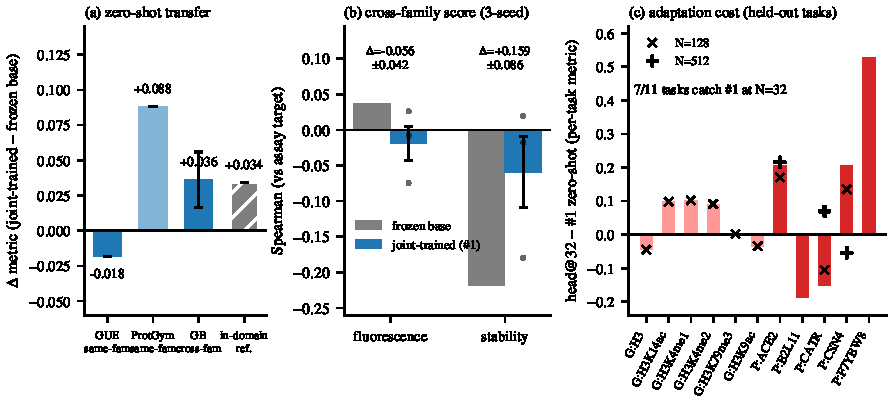
\includegraphics[width=0.90\textwidth]{fig2_transfer.pdf}
\caption{\textbf{Three operational tests of the shared scorer's claimed advantages.}
(a) Zero-shot transfer to same-family held-out tasks is a wash (GUE $-0.018$,
ProtGym $+0.088$); cross-family transfer on GenomicBenchmarks is weakly positive
($+0.036$, SEM over 3 seeds), comparable to the in-domain reference ($+0.034$;
full2 configuration, not strictly matched).
(b) Cross-family \emph{score} transfer (TAPE, 3 seeds) does not hold: fluorescence
degrades ($\Delta=-0.056\pm0.042$); stability's apparent gain
($+0.159\pm0.086$) is regression of a pathological frozen baseline ($-0.218$)
toward zero --- trained absolute Spearman stays negative ($-0.059$).
(c) Adaptation cost: a fresh \#2 linear head catches \#1's zero-shot on 7/11
held-out tasks with only $N{=}32$ labels ($\times$: $N{=}128$, $+$: $N{=}512$).}
\label{fig:transfer}
\end{figure*}

\paragraph{(a) Same-family zero-shot.}
Held-out tasks from families already in training (16 GUE + 20 ProteinGym tasks unseen by
the 37-task joint model): \arch{1}-trained $\approx$ \arch{1}-frozen base (GUE accuracy
0.496 vs 0.515, $\Delta=-0.018$; per-task 11 wins / 9 ties / 13 losses --- a wash). Joint
training on 37 tasks did not learn a strongly transferable decision function. \arch{2}
cannot participate at all: it has no head for unseen label sets --- the qualitative
difference stands, the quantitative one does not.

\paragraph{(b) Cross-family zero-shot.}
Holding out the entire GenomicBenchmarks family (training on the other six families) and
evaluating its 8 tasks gives mean $\Delta=+0.036\pm0.034$ over 3 seeds (per-seed
$+0.038$/$-0.006$/$+0.077$) --- the same magnitude as directly training on GB in-domain
($+0.034$), hinting the gain is a generic decision improvement rather than family-specific
fitting, but the std matches the mean and per-task effects range $-0.19$ to $+0.31$.
For the \emph{score} interface, holding out TAPE (while training on the DeepSTARR and
ProteinGym score families) over 3 seeds shows no clean transfer: fluorescence degrades
($\Delta=-0.056\pm0.042$, negative in all three seeds), and stability's apparent
$+0.159\pm0.086$ is entirely regression of a pathological frozen baseline ($-0.218$) toward
zero --- the trained absolute Spearman remains negative ($-0.059$). Cross-family transfer
exists, weakly, for classification only.

\paragraph{(c) Adaptation cost.}
Freezing \arch{2}'s trained encoder and fitting a fresh linear head for each of 11 held-out
tasks (6 GUE + 5 ProteinGym) with $N$ labels: the new head catches or beats \arch{1}'s
zero-shot on \textbf{7/11 tasks at $N=32$} (\cref{tab:adapt}); \arch{1} stays ahead on 3/11
even when \arch{2} is given $N=512$; one task needs $N=512$. Family means: GUE 0.476
(zero-shot) vs 0.511 (head@32); ProteinGym $-0.024$ vs 0.095. Thirty-two labels is a trivial
cost --- the ``zero-adaptation'' selling point does not convert into a meaningful
performance-or-cost advantage.


\paragraph{(d) Noul phrasing on stable checkpoints.}
Candidate text is an inference-time degree of freedom that \arch{1} has and \arch{2} cannot
have. A controlled ablation (same checkpoint, only the rendered candidate text varies; six
phrasings) on the earlier single checkpoint had suggested raw ``no/yes'' beats the redundant
``false: no / true: yes'' by $+0.066$ AUROC. Re-running on three retrained seed-averaged
stable checkpoints (\cref{fig:ablation}a) \emph{reverses} the direction: the redundant
prefix form wins on all three seeds ($0.553\pm0.023$ vs the trained phrasing's
$0.508\pm0.024$), and \textbf{no phrasing reaches \arch{2}} (best 0.553 vs 0.629). Two
conclusions: the noul deficit of \arch{1} is not a phrasing artifact (the main result is
reinforced), and even inference-level ``clean controlled'' evidence is checkpoint-dependent
--- ablations need multi-checkpoint confirmation too.

\subsection{Training dynamics}
\label{sec:dynamics}

\begin{figure*}[t]
\centering
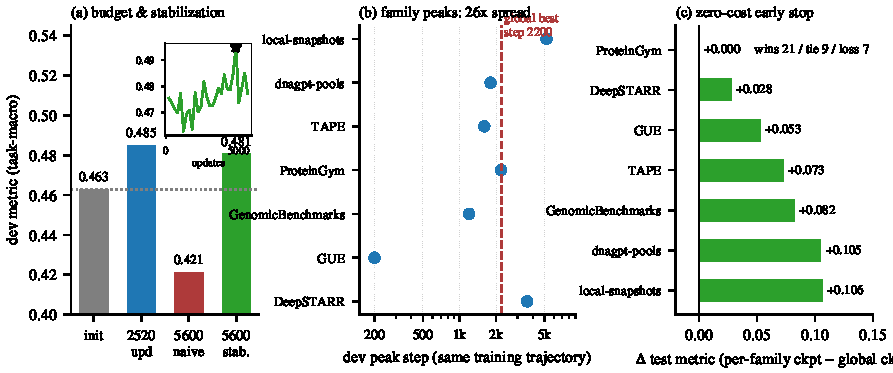
\includegraphics[width=0.90\textwidth]{fig3_dynamics.pdf}
\caption{\textbf{Training dynamics under joint multi-task fitting.}
(a) Naive budget scaling destabilizes: 5{,}600 updates score \emph{below} init
(0.421) while 2{,}520 reaches 0.485; stabilization (warmup 0.15, grad clip 0.5,
dev early stop) recovers 0.481 at 5{,}600 --- a plateau, not overfitting
(inset: stabilized dev curve; star = selected checkpoint).
(b) Family-optimal dev peaks on the \emph{same} trajectory span steps 200--5{,}200
(26$\times$), while the global best sits at 2{,}200.
(c) Per-family early stopping (zero inference-time cost) dominates at family level
(all $\Delta\ge0$, mean $+0.063$); per task: 21 win / 9 tie / 7 loss vs the global
checkpoint.}
\label{fig:dynamics}
\end{figure*}

\paragraph{Budget scaling is negative.}
On the same 43-task set, doubling updates 2{,}520$\to$5{,}600 (and per-task data
768$\to$2048) drops classification accuracy 0.485$\to$0.421 --- \emph{below} the untrained
init (0.463) --- and TAPE Spearman 0.237 $\to$ $-0.020$. Diagnosis: training loss plateaus at
${\sim}1.06$ after ${\sim}900$ steps, gradient median stays ${\approx}0.25$ for 4{,}700
further steps with early spikes (max 547), and fold classification never leaves chance
(train loss $\approx\ln 7$ throughout). This is joint-optimization instability landing in
bad basins, not overfitting: the training loss never approaches zero.

\paragraph{Stabilization repairs, and confirms a plateau.}
Warmup 0.05$\to$0.15, clip 1.0$\to$0.5, and dev early stopping (every 200 steps,
best-dev promotion) recover the 5{,}600-update budget to 0.481 --- statistically the small
budget's 0.485 (gain vs init $+0.049\approx+0.050$). Beyond ${\approx}2{,}500$ updates,
compute is not the bottleneck; the ceiling is capacity/interference of joint multi-task
training (\cref{fig:dynamics}a).

\paragraph{Per-family early stopping is free.}
On one training trajectory, family-optimal dev peaks span steps 200 (GUE) to 5{,}200
(local snapshots) --- a $26\times$ spread --- while the global best sits at 2{,}200.
Selecting each family's own best-dev checkpoint dominates the single global checkpoint at
family level (all $\Delta\ge0$; mean $+0.063$; per task 21/9/7 wins/ties/losses;
\cref{fig:dynamics}b,c), at zero inference-time cost. Part of the plateau was a
checkpoint-selection compromise, not pure capacity.

\subsection{Controlled mechanism ablations}
\label{sec:ablations}


Beyond the phrasing ablation of \cref{sec:value}d (candidate surface form is a real but
run-dependent degree of freedom, and no phrasing closes the noul gap), one more probe
concerns frozen candidate-likelihood scoring: on a multimodal route-A pilot (synthetic
property maps, frozen Qwen2.5-VL \citep{bai2025qwen25vl}), plain candidate likelihood
collapses to one class (accuracy 0.040 $<$ chance), while \emph{contrastive decoding}
$\log p(\text{cand}\mid\text{img},q)-\log p(\text{cand}\mid q)$
\citep[cf.][]{leng2024vcd,li2023contrastive} restores multi-class predictions but stays at
chance (\cref{fig:ablation}b). The reusable lesson: frozen-VLM candidate-likelihood
evaluation should default to contrastive decoding; the route itself is rejected
(\cref{app:vlm}).

\section{Discussion and Limitations}
\label{sec:discussion}

\paragraph{When would a shared typed-decision scorer win?}
Within our evidence: not on seen tasks, not zero-shot (at base level), weakly on
cross-family classification only, and its zero-adaptation edge is erased by ${\approx}32$
labels. What survives unambiguously is the interface itself: no task parameters, arbitrary
dynamic candidates, immediate inference on new tasks (\arch{2} architecturally cannot), and
inference-time degrees of freedom (phrasing, per-family checkpoints) --- though the 3-seed
ablation shows phrasing tuning does not close the noul gap ($0.553<0.629$). Deployment
regimes with very large or open candidate sets, frequent task arrivals, or true
zero-label cold starts may shift the balance; those are hypotheses, not our results.

\paragraph{Absolute levels vs.\ specialized anchors.}
Joint-37 choice ${\approx}0.49$ and score ${\approx}0.01$--$0.02$ sit far below
specialized training: the same architecture family reaches 87--89\% on promoters, 56--58\%
on fold class and GFP MAE 0.32--0.49 under per-task recipes \citep{wang2024llamagene}. The
joint regime is a deliberate stress test (one checkpoint serving 37 heterogeneous tasks,
$\le2048$ samples each, ${\approx}70$ updates per task); it calibrates ``where shared
decision interfaces currently stand under multi-task small budgets'' and is not an
architecture ceiling.

\paragraph{Threats to validity.}
(i) The head-to-head uses a 37-task slice (PG/GUE capped at 12), not all 290: the benchmark
is the infrastructure contribution and the comparison is a matched slice --- we state the
two scopes separately everywhere. (ii) 3 seeds; SEM is across tasks, run-std across seeds;
noul ($n{=}7$) and score ($n{=}9$) have few tasks. (iii) \arch{3} is not matched (frozen,
different backbone, truncation, different score protocol). (iv) The cross-family score arm
now has 3 seeds, but with $n{=}2$ tasks the stability $\Delta=+0.159$ depends on the
pathological frozen baseline and must be read with that caveat (\cref{sec:value}). (v) dev
selection noise is mitigated (96$\to$256 samples) but not eliminated. (vi) GPU
nondeterminism is irreducible; only seed averaging absorbs it. (vii) the 512-token budget
excludes long-sequence examples (exclusion rates reported, never silent truncation).


\section{Conclusion}
\label{sec:conclusion}

We introduced BioDecisionBench --- 290 biological sequence decision tasks from 10 source
families, three modalities and four typed decision primitives, under one record format and
a leak-proof admission protocol (zero within-task leakage after isolation; conflict groups
quarantined, legacy blind tests preserved verbatim) --- together with reproducible
build/evaluation/training code. On its 37-task matched slice, the first seed-averaged
three-way architecture comparison gives a bounded, honest answer: the shared typed-decision
scorer does not beat per-task heads (significantly worse noul, parity elsewhere, less
stable), its zero-shot and cross-family transfer are weak, and its zero-adaptation claim is
matched by a 32-label fresh head. Its real value is the interface: dynamic candidates, no
task parameters, immediate new-task inference. Methodologically, we documented a complete
conclusion-reversal case from run variance ($\pm0.05$--$0.1$) and propose seed averaging,
run-std reporting and stabilized selection as the minimum bar for architecture comparisons
in this regime. Future work: per-family training over all 290 tasks, per-task early
stopping, a matched generative arm (fine-tuned small LM), real-image multimodal evaluation,
and re-testing transfer at larger budgets and backbones.


\bibliographystyle{plainnat}
\bibliography{references}

\appendix
\section{Full per-family results}
\label{app:full}

\Cref{tab:appendix} reports per-family, per-seed means for the two trained arms.
% Table 4: appendix per-family comparison (generated by gen_tables.py; seed-avg of per-task metrics)
\begin{table}[t]
\centering
\caption{Per-family, per-seed means for the two trained arms (task-macro of per-task seed means). \#1 uses per-family early-stop checkpoints (37-task slice; families as in the training scheduler), \#2 the full-run checkpoint. DeepLoc (multi\_noul) and double-sequence tasks are outside this harness.}
\label{tab:appendix}
\footnotesize
\begin{tabular}{llccc}
\toprule
Family & Primitive & \#1 (mean$\pm$std over 3 seeds) & \#2 & n \\ \midrule
DeepSTARR & score & 0.035$\pm$0.027 & 0.053$\pm$0.023 & 3 \\
GUE & choice & 0.464$\pm$0.017 & 0.478$\pm$0.013 & 3 \\
GenomicBenchmarks & choice & 0.402$\pm$0.082 & 0.305$\pm$0.014 & 3 \\
GenomicBenchmarks & noul & 0.478$\pm$0.017 & 0.629$\pm$0.005 & 3 \\
ProteinGym & score & 0.015$\pm$0.058 & 0.022$\pm$0.015 & 3 \\
TAPE & score & -0.014$\pm$0.047 & -0.027$\pm$0.043 & 3 \\
dnagpt\_pools & choice & 0.519$\pm$0.006 & 0.514$\pm$0.030 & 3 \\
local\_snapshots & choice & 0.534$\pm$0.016 & 0.536$\pm$0.030 & 3 \\
\bottomrule
\end{tabular}
\end{table}


\section{Adaptation cost and ablation tables}

% Table 3: adaptation cost (generated by gen_tables.py)
\begin{table}[t]
\centering
\caption{Adaptation cost on 11 held-out tasks: \#1 zero-shot (no labels, no training) vs \#2 new linear head fitted on $N$ labels (frozen shared encoder). \#2 catches or beats \#1's zero-shot on 7/11 tasks already at $N{=}32$.}
\label{tab:adapt}
\footnotesize
\begin{tabular}{llcccc}
\toprule
Task & Metric & \#1 zero-shot & \#2 $N{=}32$ & $N{=}128$ & $N{=}512$ \\
\midrule
gue\_H3 & accuracy & 0.555 & 0.510 & 0.510 & -- \\
gue\_H3K14ac & accuracy & 0.445 & 0.543 & 0.543 & -- \\
gue\_H3K4me1 & accuracy & 0.430 & 0.532 & 0.532 & -- \\
gue\_H3K4me2 & accuracy & 0.450 & 0.541 & 0.541 & -- \\
gue\_H3K79me3 & accuracy & 0.490 & 0.492 & 0.492 & -- \\
gue\_H3K9ac & accuracy & 0.485 & 0.451 & 0.451 & -- \\
pg\_ACE2\_HUMAN\_Chan\_2020 & spearman & -0.176 & 0.029 & -0.005 & 0.040 \\
pg\_B2L11\_HUMAN\_Dutta\_2010\_binding-Mcl-1 & spearman & 0.133 & -0.054 & -- & -- \\
pg\_CATR\_CHLRE\_Tsuboyama\_2023\_2AMI & spearman & 0.066 & -0.086 & -0.039 & 0.135 \\
pg\_CSN4\_MOUSE\_Tsuboyama\_2023\_1UFM & spearman & -0.034 & 0.171 & 0.101 & -0.088 \\
pg\_F7YBW8\_MESOW\_Ding\_2023 & spearman & -0.112 & 0.416 & -- & -- \\
\bottomrule
\end{tabular}
\end{table}



\begin{figure*}[t]
\centering
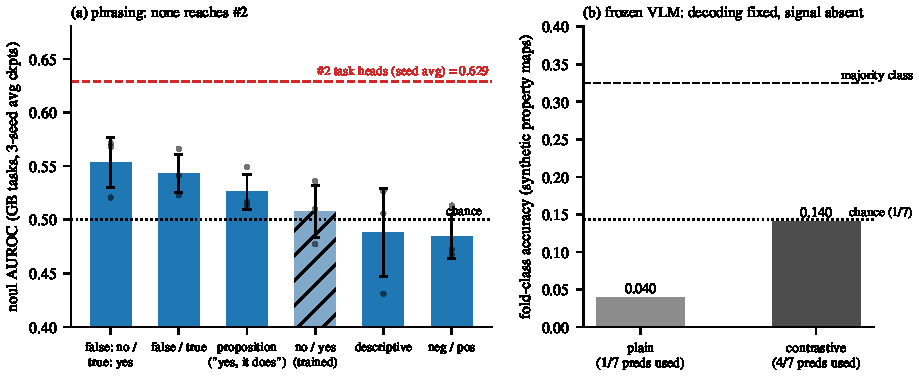
\includegraphics[width=0.98\textwidth]{fig4_ablation.pdf}
\caption{\textbf{Controlled mechanism ablations.}
(a) Noul candidate phrasing on three seed-averaged stable checkpoints (same
weights; only candidate text varies). No phrasing reaches the per-task-head
reference (0.629, dashed); the best (``false: no / true: yes'', $0.553\pm0.023$)
beats the \emph{trained} phrasing (hatched) on all three seeds --- reversing the
single-checkpoint finding, i.e., inference-level ablations are also
checkpoint-dependent.
(b) Frozen VLM on synthetic property maps (multimodal route-A pilot): plain
candidate likelihood collapses to one class (acc 0.040, 1/7 classes used);
contrastive decoding removes the collapse (0.140, 4/7) but remains at chance ---
decoding fixed, signal absent.}
\label{fig:ablation}
\end{figure*}

\label{app:ablations}

% Table 5: noul phrasing x 3 stable checkpoints (gen_tables.py)
\begin{table}[t]
\centering
\caption{Noul AUROC on GB tasks for six candidate phrasings, evaluated on three seed-averaged stable checkpoints (same weights per column; only rendered candidate text varies). No phrasing reaches the per-task-head reference (0.629). The trained phrasing is marked \dag.}
\label{tab:phrasing}
\small
\begin{tabular}{lcccc}
\toprule
Phrasing & s1 & s2 & s3 & mean$\pm$std \\ \midrule
false: no / true: yes & 0.572 & 0.568 & 0.521 & 0.553$\pm$0.023 \\
false / true & 0.566 & 0.523 & 0.541 & 0.543$\pm$0.018 \\
proposition (``yes, it does'') & 0.517 & 0.513 & 0.549 & 0.526$\pm$0.016 \\
no / yes (trained)$^\dagger$ & 0.477 & 0.536 & 0.510 & 0.508$\pm$0.024 \\
descriptive & 0.527 & 0.506 & 0.431 & 0.488$\pm$0.041 \\
neg / pos words & 0.513 & 0.468 & 0.472 & 0.484$\pm$0.020 \\
\bottomrule
\end{tabular}
\end{table}

% Table 6: TAPE cross-family score arm, 3 seeds (gen_tables.py)
\begin{table}[t]
\centering
\caption{Cross-family score transfer (TAPE held out; DeepSTARR and ProteinGym score families in training). Spearman per seed; ``abs'' = trained absolute value. Stability's positive $\Delta$ reflects a pathological frozen baseline ($-0.218$) regressing toward zero, not genuine transfer.}
\label{tab:tape}
\small
\begin{tabular}{llccccc}
\toprule
Task & & frozen & tr.\ s1 & tr.\ s2 & tr.\ s3 & $\Delta$ mean$\pm$std \\ \midrule
tape\_fluorescence & abs & 0.037 & -0.008 & 0.026 & -0.075 & -0.056$\pm$0.042 \\
tape\_stability & abs & -0.218 & -0.018 & 0.020 & -0.179 & +0.159$\pm$0.086 \\
\bottomrule
\end{tabular}
\end{table}


\section{Multimodal route-A pilot}
\label{app:vlm}

Protein sequences without resolved structures were rendered as synthetic
amino-acid property heatmaps (7 normalized physicochemical tracks $\times$ position,
matplotlib viridis) and presented to a frozen Qwen2.5-VL-3B \citep{bai2025qwen25vl}
alongside the fold-class question. Plain full-candidate likelihood collapsed to a single
candidate on all 200 images (accuracy 0.040; macro-F1 0.011; 1/7 classes predicted) ---
candidate text priors dominate and the image does not change the ranking. Contrastive
decoding, $\log p(\text{cand}\mid\text{img},q)-\log p(\text{cand}\mid q)$, restores
multi-class behavior (4/7 classes, accuracy 0.140) but sits at chance
($1/7=0.143$), far below the majority baseline (0.325) and the text-only frozen LM
(0.320). Image sanity checks rule out rendering failure (per-image statistics and
cross-image correlations normal). Conclusion: route A (synthetic renders) with a frozen
VLM is a dead end; the reusable finding is that \emph{frozen-VLM candidate-likelihood
evaluation should default to contrastive decoding}. Real-image localization (HPA) and
fine-tuned VLM arms are a separate work.

\section{Data, licensing, and disclosures}

\paragraph{Data and licensing.}
All sources are public datasets with license, revision and SHA-256 recorded in download
receipts; no human-subject data. RNAcompete is the 14-RBP test subset (not the full
${\sim}$200); DeepGOZero/PEER/DeepSEA remain in the catalog as needs-upstream-work and are
not claimed as coverage. The splice label-convention doubt (\cref{sec:admission}) is
explicitly recorded for independent verification.

\paragraph{LLM-use disclosure.}
[To be finalized per venue checklist: writing assistance disclosure.]
\section{Reproducibility}
\label{app:repro}

Every figure and table regenerates from on-disk JSONs via one script per artifact
(\texttt{paper\_v2/figures/gen\_*.py}); no metric is hardcoded in the plotting or table
code. Each run persists \texttt{run\_config.json} (flags, seeds, caps),
\texttt{train\_trace.jsonl} (per-step loss/grad) and \texttt{dev\_curve.jsonl} (per-family
dev scores); evaluation subsets are drawn with a fixed sampling seed (20261001) rather than
first-$N$ --- a bug we found and fixed: class-ordered test files plus first-$N$ sampling
produced a spurious noul AUROC of 0.387 that looked like a polarity bug but was a sampling
artifact. Hardware: single H20/A800-class GPU per run; nondeterminism is absorbed by the
seed protocol of \cref{sec:seedavg}.


\end{document}
